\section{Raytracing}
 
\begin{figure}[H]
    \centering
    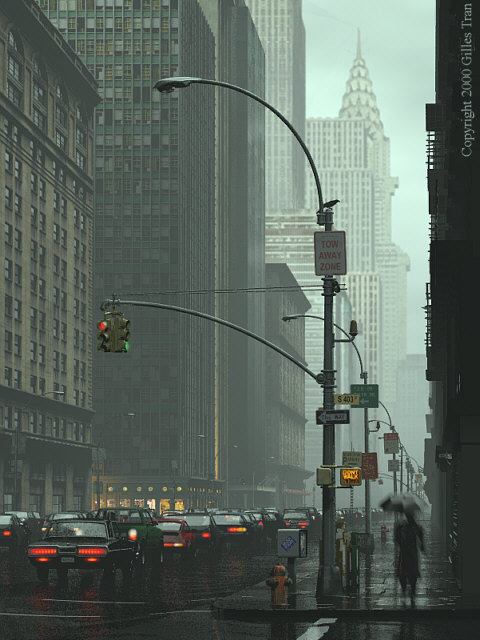
\includegraphics[height=0.7\textwidth]{images/mouille.jpg}
    \caption{Ein mit Povray gerendertes Bild aus dem Jahre 2000.}
    \label{fig:povray}
\end{figure}


 \begin{figure}[H]
    \centering
    
\includegraphics[height=0.5\textwidth]{images/vray.png}
    \caption{Ein mit VRay gerendertes Bild aus dem Jahre 2015.}
    \label{fig:cray}
\end{figure}


 \begin{figure}[H]
    \centering
    
\includegraphics[height=0.5\textwidth]{images/freestyle.jpg}
    \caption{Ein nicht photorealistisches Rendering in Blender aus dem Jahre 2015.}
    \label{fig:cray}
\end{figure}


 \begin{figure}[H]
    \centering
    
\includegraphics[height=0.5\textwidth]{images/pixar.jpg}
    \caption{Ein nicht photorealistisches Rendering mit Pixar's renderman aus dem Jahre 2001.}
    \label{fig:cray}
\end{figure}

\subsection{Farbwahrnehmung und Farbmodelle}

\subsection{Globale Beleuchtungsmodelle und Rendergleichung}

\subsubsection{Sphären, Raumwinkel und infinitessimale Flächenstücke}

 \begin{figure}[H]
    \centering
    
\includegraphics[width=0.7\textwidth]{images/solidangle.png}
    \caption{Raumwinkel}
    \label{fig:cray}
\end{figure}

\subsubsection{Photometrie}

Die Radiantenergie $Q$ ist die Lichtenergie. Sie wird durch einen Strom von Photonen erzeugt. Die Energie eines Photons ist 
durch $E=h \cdot f$ geben, wobei $h$ das konstante Planksche Wirkungsquantum und $f$ die Frequenz der Welle ist (Welle-Teilchen Dualismus).  

\begin{Definition}
Die Ableitung nach der Zeit
\begin{align}
\phi := \frac{\partial Q}{\partial t}
\end{align}
wird als Radiant Flux oder Strahlungsleistung bezeichnet. Die Einheit ist Watt (W).
Diese  beschreibt den Energiefluss, beziehungsweise den Energie-Eintritt und Energie-Austritt.
\end{Definition}

 \begin{figure}[H]
    \centering
    \includegraphics[height=0.5\textwidth]{images/infrared_dog.jpg}
    \caption{Strahlungsleistung an verschiedenen Punkten der Oberfläche}
    \label{fig:cray}
\end{figure}


\begin{Satz}

Das sogenannte photometrische Grundgesetzt beschreibt die Strahlung, die von einem  Flächenelement auf ein anderes  Flächenelement 
übertragen wird.  
 \begin{figure}[H]
    \centering
    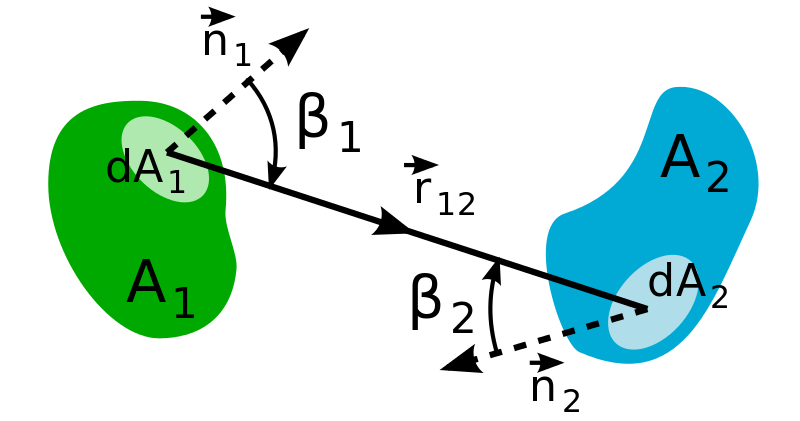
\includegraphics[width=0.7\textwidth]{images/Fotometrisches_Grundgesetz_Schema.png}
    \caption{Fotometrisches Grundgesetz}
    \label{fig:cray}
\end{figure}

\begin{align}
\phi &= \int_{A_1} \int_{\pi_s(A_2)} L(x, \omega)\cdot \cos(\beta_1) \cdot dA_1 \cdot d \omega \\
&= \int_{A_1} \int_{A_2} \frac{1}{r_{12}^2}  \cdot L(x, \omega) \cdot \cos(\beta_1) \cdot \cos(\beta_2) \cdot dA_1 \cdot d A_2 \; .
\end{align}
Hierbei ist $L(x, \omega)$   die Radiance oder auch Stahldichte  der von $A_2$ abgestrahlte Strahlung  und ist (formal) durch  
\begin{align}
L(x, \omega) := \frac{d^2 \phi}{\cos(\omega) \cdot dA \cdot d\omega} \; ,
\end{align}
wobei $\theta$ der Winkel zwischen der Flächennormale am Punkt $x$ und der Richtung $\omega$ ist.
Die Radiance ist also der Radiant Flux pro infinitesimale Flächeneinheit $dA$ und pro  Raumwinkel $d \omega$ unabhängig vom Strahlwinkel $\cos(\theta)$.
Die Einheit ist $\frac{W}{m^2\cdot sr}$ (Watt ($W$) pro Quadratmeter ($m^2$) und pro Steradiant ($sr$)). 
Mit $L_i, L_o,Lr,L_e$ bezeichnet man entsprechend den eintreffende, ausgehende, reflektierte beziehungsweise emittierte Radiance.
\end{Satz}

\begin{Definition}
Eine Objekt, dessen Stahldichte für alle Punkte und Richtungen konstant ist, also
$L(x, \omega) = c$  für alle $x \in O$ und $\omega \in S^2$, bezeichnet man auch als Lambertschen Strahler. 
\end{Definition}

\begin{Definition}
Die Irradiance $E$ ist definiert durch
\begin{align}
E(x) := \int_{S^2} L_i(x, \omega) \cos{\theta_i} d\omega_i \; ,
\end{align}
also die auftreffende Strahlungsleistung pro Flächeneinheit. 
\end{Definition}

\begin{Definition}
Die Radiocity $B$ ist definiert durch
\begin{align}
B(x) := \int_{S^2} L_o(x, \omega) \cos{\theta_i} d\omega_i \; ,
\end{align}
also die ausghende Strahlungsleistung pro Flächeneinheit. 
\end{Definition}



\begin{Definition}
Die  bidirektionale Reflektanzverteilungsfunktion (engl. Bidirectional Reflectance Distribution Function, BRDF)
ist eine Funktion $f_r (x, \omega_i, \omega_r)$, die das Reflexionsverhalten der Oberfläche eines Materials beschreibt. 
Sie hat als Eingabe die ausgehende Richtung $\omega_r$ und die eingehende Richtung  $\omega_i$ am Punkt $x$. 
Sie  liefert den Quotienten aus Strahlungsdichte und Bestrahlungsstärke für die ausgehende Richtung $\omega_r$ und die eingehende Richtung  $\omega_i$ am Punkt $x$.
Sie gibt somit die Abhängigkeit des reflektierten Lichts von der einfallenden Lichtstärke an: 
\begin{align}
L_r(x, \omega_r) = \int_{S^2}f_r (x, \omega_i, \omega_r) \cdot L_i(x, \omega_i) \cdot  \cos(\theta_i) d\omega_i
\end{align}
Letztere Gleichung wird  Reflectance-Gleichung genannt.
\end{Definition}
 \begin{figure}[H]
    \centering
    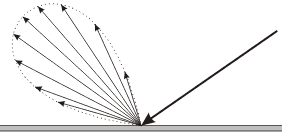
\includegraphics[width=0.6\textwidth]{images/brdf2.png}
    \caption{BRDF Funktion}
    \label{fig:raytracin_brdf}
\end{figure}


 
\subsubsection{Die Rendergleichung (Erste und zweite Form)}

Durch Hinzunahme des von dem Oberflächenpunkt emittierten Lichtes $L_e(x, \omega_o)$ zu dem   an diesem Punkt reflektiert Lichtes erhalten wir die sogenannte Renderingleichung 
\begin{align}
L_o(x, \omega_o) = L_e(x, \omega_o)  + \displaystyle \int_{S^2}f_r (x, \omega_i, \omega_0) \cdot L_i(x, \omega_i)  \cdot  \cos(\theta_i) d\omega_i \; ,
\end{align}
wobei $L_e(x, \omega_o)$ die von der Oberfläche emittierte Strahlungsleistung ist. 

Definiert man die Menge $\Omega$  als die Menge aller Flächen (Dreiecke) in der Szene und
\begin{align}
V(x,y) := \begin{cases}
1 \text{ falls } \overline{xy} \cap \Omega = \emptyset \\
0 \text{ sonst }
\end{cases}
\end{align}
so gilt die Beziehung $L_i(x, \omega_i) = V(x,y) \cdot L_o(x, \omega_i)$.
Zusammen mit der Beziehung $d\omega =  \frac{1}{||x -y||^2} \cdot  \cos(\theta_y)$ und der Definition 
\begin{align}
G(x,y) := V(x,y)  \frac{ \cos(\theta_y) \cdot  \cos(\theta_i)}{||x -y||^2} 
\end{align}
erhält man die Rendergleichung in zweiter Form 
\begin{align}
L_o(x, \omega_o) = L_e(x, \omega_o)  + \displaystyle \int_{\Omega} f_r (x, \omega_i, \omega_o) \cdot   L_o(y, \omega_i)  \cdot  G(x,y) \cdot   d\omega_i \; .
\end{align} 


\subsection{Raycasting}
\subsection{"Klassisches" Raytracing}
Das klassische Raytracing nach Whitted ist durch folgenden rekursiven Algorithmus gegeben:
\begin{itemize}
\item d
\end{itemize}
\subsection{Radiocity Verfahren}
 \begin{figure}[H]
    \centering
    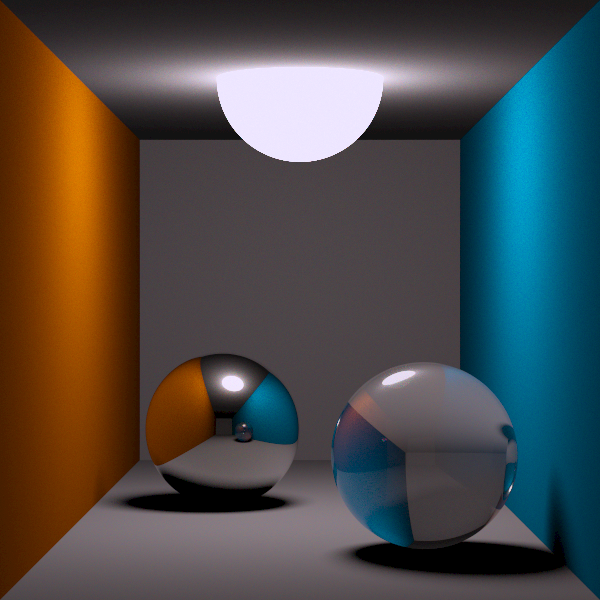
\includegraphics[width=0.7\textwidth]{images/diffus.png}
    \caption{Rein diffuses beleuchtungsmodell}
    \label{fig:diffus}
\end{figure}

\subsection{Pathtracing}
\subsubsection{Wahrscheinlichkeitstheorie und Monte Carlo Integration}  
Ein Wahrscheinlichkeitsraum ist ein Tripel $(\Omega, \Sigma, \mathbb{P})$ bestehend aus
\begin{itemize}
\item Einer Menge $\Omega$
\end{itemize}


\begin{Definition}
Ist $X$ eine kontinuierliche Zufallsvariable mit Wahrscheinlichkeitsdichte $\rho: \Omega \to [0,1]$, dann heißt
\begin{align}
\mathbb{E}[X] := \int_{\Omega} \omega \cdot \rho(\omega) d\omega \; ,
\end{align}
beziehungsweise für eine Funktion $f: \Omega \to \mathbb{R}$
\begin{align}
\mathbb{E}[f(X)] := \int_{\Omega} f(\omega) \cdot \rho(\omega) d\omega \; .
\end{align}
\end{Definition}


\begin{Satz}[Gesetzt der großen Zahlen]
Ist $X$ eine kontinuierliche Zufallsvariable mit Wahrscheinlichkeitsdichte $\rho: \Omega \to [0,1]$ und $f: \Omega \to \mathbb{R}$, so gilt:
\begin{align}
\frac{1}{N} \sum_{i= 0}^{N} f(\omega_i) \xrightarrow{ N \to \infty } \mathbb{E}[f(X)] \text{ (in Wahrscheinlichkeit)}
\end{align}
\end{Satz}
\begin{figure}[H]\centering
    \subfloat[Pathtracing mit wenig Samples]{
        \hspace*{0.05\textwidth}
    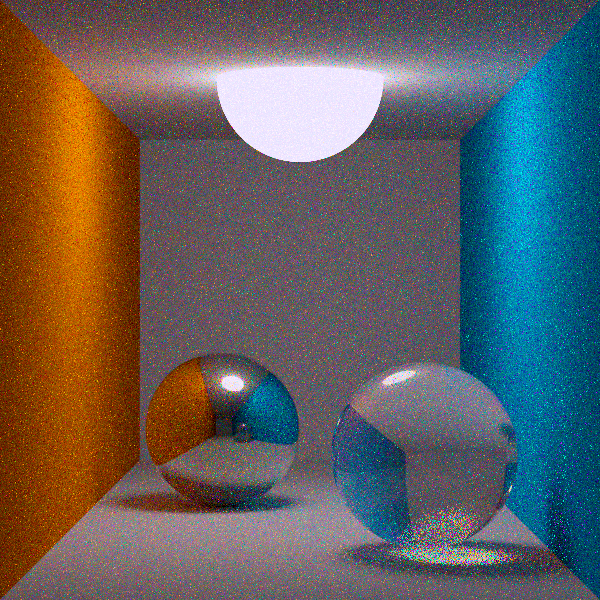
\includegraphics[width=0.5\textwidth]{images/Path_Tracing_Low.png}
        \hspace*{0.05\textwidth}
        \label{fig:closed-mesh-gender0}
    }
    \hspace*{0.1\textwidth}
    \subfloat[Pathtracing mit vielen Samples]{
    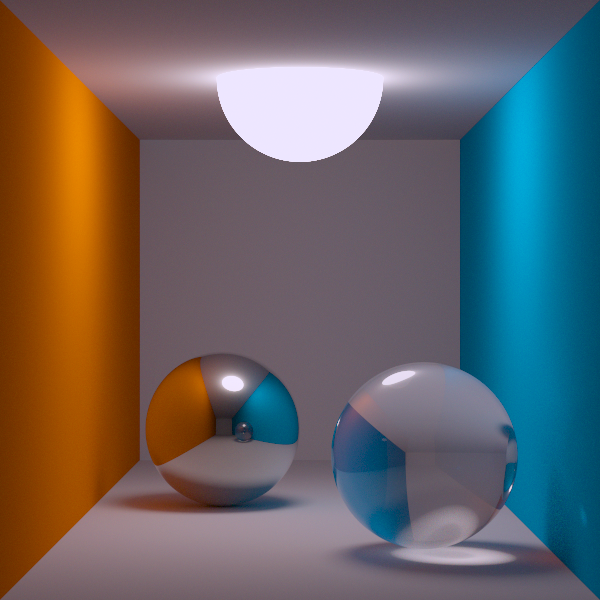
\includegraphics[width=0.5\textwidth]{images/Path_Tracing_High.png}
        \label{fig:closed-mesh-gender1}
    }
\end{figure}

\subsubsection{Raymarching}
\subsection{Klassifikation der Verfahren}

\subsection{Datenstrukturen für Bereichsabfragen}


\subsection{Labor}
\subsubsection{Blender}
\subsubsection{Echtzeitfähiges Raymarching in WebGL}
